\documentclass[]{article}

\usepackage{graphicx}
\usepackage{url}
\usepackage{algorithm}

\newcommand{\comment}[1]{}

\title{CS252: An Example Project Report}
\author{
\begin{tabular}{cc}
	Bhavishya Mittal & Javesh Garg \\
	11198 1 & 11334 \\
	\url{bhavishy@iitk.ac.in} & \url{javeshg@iitk.ac.in} \\
	\multicolumn{2}{c}{Indian Institute of Technology, Kanpur}
\end{tabular}
}
\date{Final report \\
15th April, 2013}	

\begin{document}

\maketitle

\begin{abstract}
	Lets You Manage the Conferences by showing the important links related to that conference (submissions and call for papers) and 
	tells about the submission deadlines. It is basically a crawler developed in python (using urllib2 module) \cite{urllib2}.
\end{abstract}

\section{Problem Statement}

You want to keep track of certain conferences.You may only know the short acronym of the conference or the full name. Any extra information about the topic of the conference may also be provided. So, we need to develop a web crawler for the purpose, which will show the deadline for the various conferences. The users enters the details of the conference as specified above and the programme returns the deadline for the conference along with some links for webpages it consider useful.

\section{Method Used}
The programme is a basic implementation of a back-end database and a web-crawler. Whenever a query is made, the programme first searches an indexed database for a fresh result. The database stores the results along with a timestamp as to when the result was stored.
If found and is not more than a week long ago, then it shows the result from the database itself. Else it searches web using 'ajax.googleapis.com' \cite{ajax} which returns a JSON file with eight URL's. The crawler reads that file and finds out if the first URL is worth crawling(i.e. not a .pdf extension or a youtube link etc.), and then crawls the interet using that URL as the base link.
The python module "urllib2.openurl()" is used to open both HTTP and HTTPS results tuneeling through a proxy server.
The crawler segregates the links as priority-links and normal-links as per priority of crawling them. The segregation is done by a searching a set of words in the URL's and the text that represents them. Also the links are stored to counter any kind of re-visits to the same pages.
If the conference deadline is found, it displays that and saves the result into the database along with the curret timestamp.

\begin{algorithm}
\caption{PSEUDO-CODE for CRAWLER}
\begin{itemize}
	\item First set proxy connection
	\item Then search for first valid page on google and supply this link to parser
	\item Save the webpage reffered to above link and parse it for all links.
	\item We have maintained two queues for maintaining url list to be parsed.These
are priority url and normal url list. Our crawler first crawls through
links in priority url and then url list.If the url or the text represent-
ing url on the webpage contains some specific keywords like conference
name,”calender”,timeline etc then the url is moved to priority list.
	\item Often ’href’ attribute has relative value or ’\#’ or ’mailto’ links. There-
fore to get par with this proper url checking and standardization has
been done ie the url is made absolute.
	\item Duplication of url is also checked.
	\item If the content of webpage, has keyword like ”important dates”,”submission
deadline” etc (not as hyper link) then we check for date pattern in next 10-20 lines. If we get one we show that date as result and stops the crawler.
\end{itemize}
\end{algorithm}


\section{Results}
The programe shows the submission deadline for the particular conference the user queried for. It takes the name or acronym of the conference and its topic (not required) as a form. On clicking the submit button the programe checks the databse or crawls the internet as per the conditions specified in the above section. It shows the deadline and some of the important links related to the submissions for the conference.

The links are mainly the first page that the crawler parsed (the base URL), the final URL from where the Deadline was found and the intermediate Priority-URL's the crawler crawled through.
If the result is not found after parsing 'Fifty' unique pages, it stops and responds "Sorry, Query Not Found".
For the various queries we searched for testing purposes and comparing of results, the crawler gave the \textbf{correct result almost "80\%" of the times} andthat too within two-three pages of the base URL selected from web search using "Google". The implementation using 'urllib2' \cite{urllib2} library is fast enough to be considered quite efficient. 

\begin{figure}
	\centering
	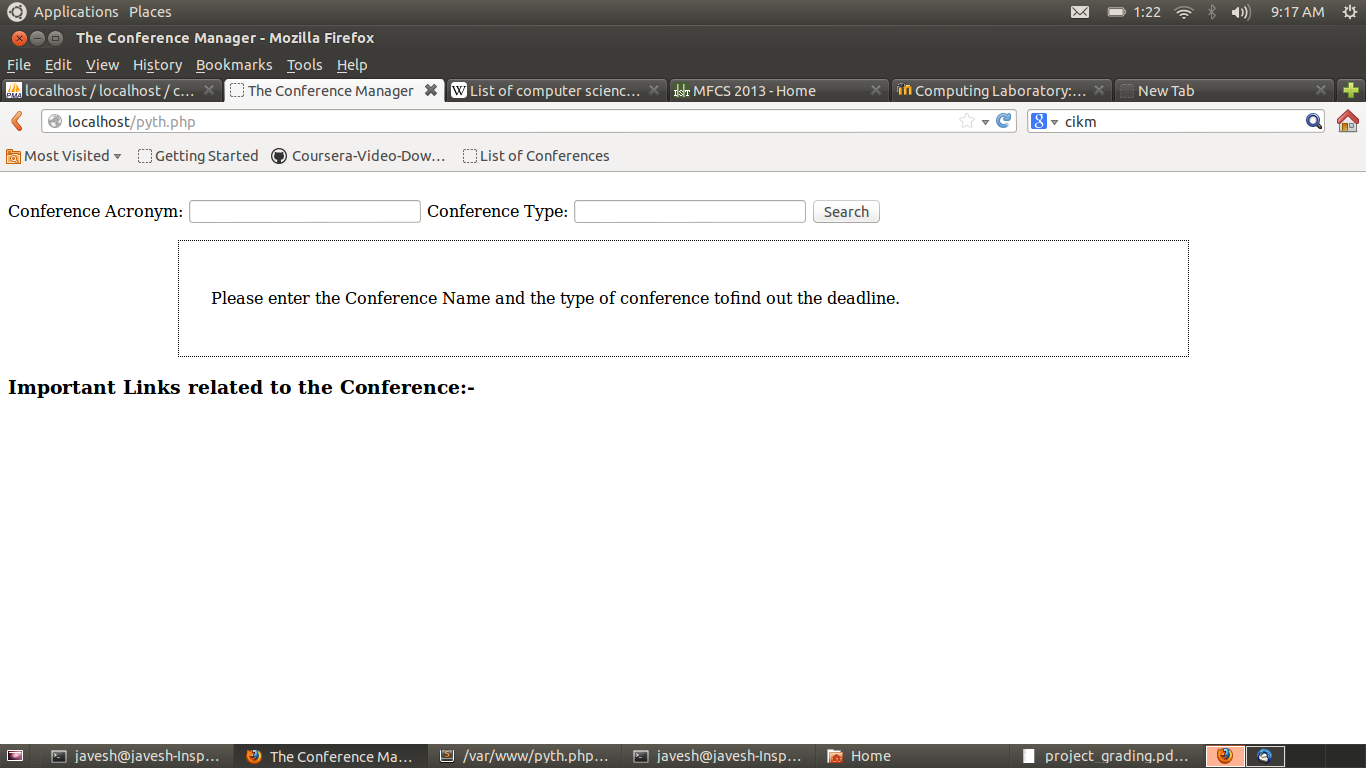
\includegraphics[width=0.95\columnwidth]{initial.png}
	\caption{Image unscrambled}
	\label{fig:block5}
\end{figure}
\begin{figure}
	\centering
	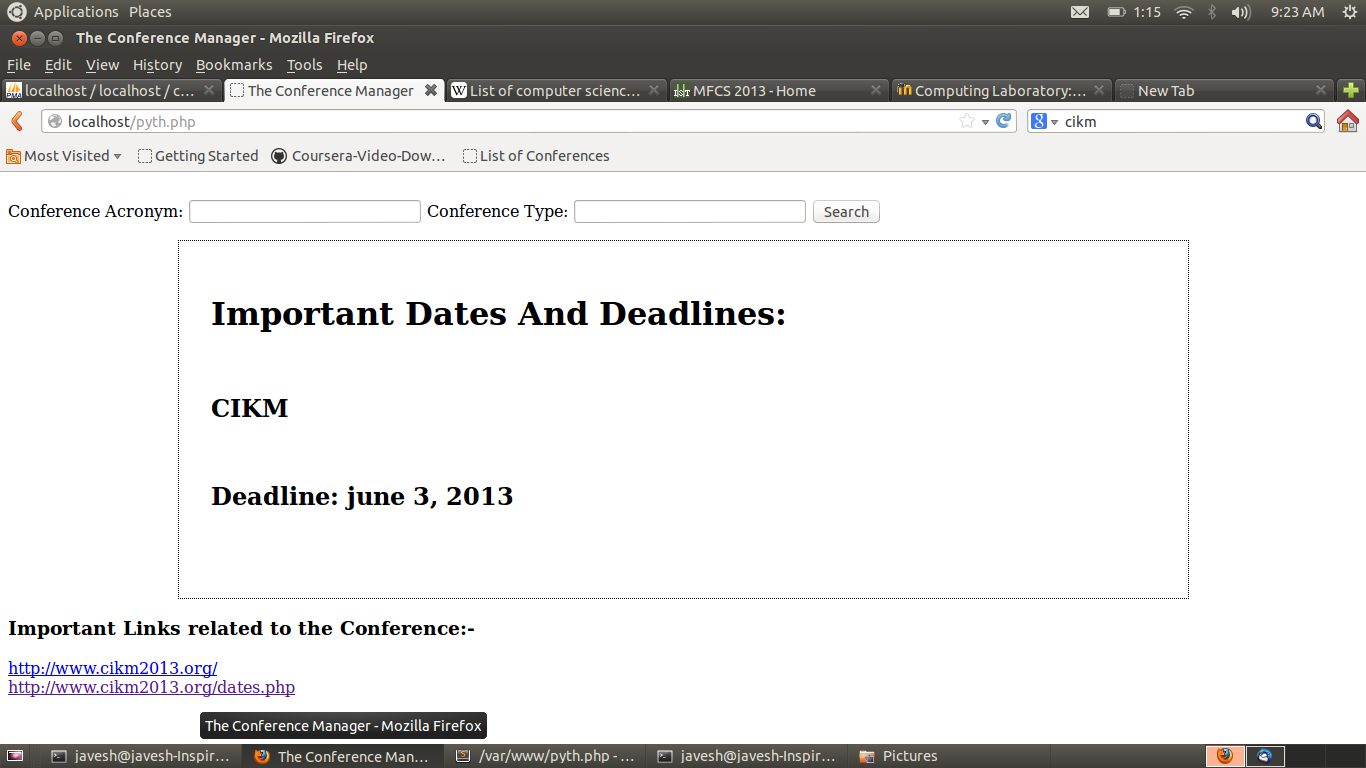
\includegraphics[width=0.95\columnwidth]{result.png}
	\caption{The final query as proccessed by the crawler.}
	\label{fig:block2}
\end{figure}

\section{Conclusions}
We developed an efficient crawler that can answer your queries regarding deaddlines for conferences. Building and efficient crawler to solve your purpose is not difficult but choosing right strategies will lead to a highly intelligent web application. Some of the most important improvements in this regard are as follows:
\begin{itemize}
	\item The first link that we get by a web search can be improved upon by NLP and machine learning. Automatic and user given error 		checking mechanism can be put up in place.
	\item As a politeness check, the robots.txt \cite{robot} file can be respected for each web site. And a dynamic list of websites can be made that 		have requested us not to crawl their servers.
	\item A dynamic and self learning mechanism can be in place which will ignore more of the extensions(like .gif, .png, .mp3, .pdf ) etc.
	\item A frequency manager can be in place which will manage the frequency of re-visits to a particular web server or website.
	\item Other features of URL normalization, Metadata export (for faster check of duplicates) and distributed crawling can be 		implemented.
\end{itemize}

\begin{thebibliography}{9}
	\bibitem{urllib2}
	\textbf{Python Docs - urllib2}\\	\url{http://docs.python.org/2/library/urllib2.html}
	\bibitem{ajax}
	\textbf{Ajax Google API}		\url{https://ajax.googleapis.com/ajax/services/search/web?v=1.0&rsz=large&q=web+crawler}
	\bibitem{robot}
	\textbf{Robots exclusion standard}	\url{http://en.wikipedia.org/wiki/Robots_exclusion_standard}
	\bibitem{parser}
	\textbf{HTMLParser module}		\url{http://docs.python.org/2/library/htmlparser.html}
	\bibitem{proxy}
	\textbf{How to tunnel through Proxy}	\url{http://docs.python.org/2/library/urllib2.html#urllib2.ProxyHandler}
\end{thebibliography}

\end{document}
